\chapter{Neural Networks}
Neural networks are machine learning algorithms inspired by the biological neural network that constitute the brain. The neural network is a collection of nodes called neurons that transmits and processes signals to and from other neurons connected to it, much like the biological neural network. The goal of a neural network is to approximate some function by learning parameters that results in the best approximation.
\\
\\
In this section we introduce the neural network...

\section{Feedforward neural networks} \label{sec:feedforward_nn}
The most simple neural networks are called feedforward neural networks or multilayer perceptrons (MLPs). They are called feedforward as information flows in one direction through the neurons. The neurons are typically arranged in layers to indicate which neurons receive and sends data to which neurons. These layers are typically vector-valued with each element of the vector playing the role as a neuron. As such one can describe a neural network as a chain of functions. Say we have 3 layers, then the neural network is $f(\mathbf{x}) = f^{(3)}\lr{f^{(2)}\lr{f^{(1)}\lr{\mathbf{x}}}}$, with $f^{(1)}$ being the first layer to pass the data, $f^{(2)}$ the second layer and so on. The final layer is called the output layer, while the intermediate layers, that don't directly show their output to the user, are called hidden layers. \\
\\
A feedfoward neural network is shown in figure \ref{fig:mlp} where the data flows from the input layer through 2 hidden layers and finally to the output layer. While the number of neurons in the input layer and output layer depends on example and label dimensions, the number of neurons in the hidden layers and also the number of hidden layers are a design decision chosen by the architect. \\
\\
The data is sent through these layers by multiplying the inputs with weights $\boldsymbol{w}$, adding a bias $\boldsymbol{b}$ and finally applying an activation function $g$ to the result. An activation function is a non-linear function that makes it so we don't just pass linear transformations of the examples through the network, so that we can actually learn non-linear functions. Activation functions come in many different kinds, some of the most popular can be seen in figure \ref{fig:act_funcs}. For a network with 2 hidden layers the result of the first hidden layer is $f^{(1)}\lr{\boldsymbol{X}} = g_1 \lr{\boldsymbol{X} \boldsymbol{w}_1 + \boldsymbol{b}_1}$ and the result of the second hidden layer is $f^{(2)} \lr{f^{(1)}\lr{\boldsymbol{X}}} = g_2 \lr{f^{(1)}\lr{\boldsymbol{X}} \boldsymbol{w}_2 + \boldsymbol{b}_2}$. The subscripts indicate that the activation functions, weights and biases are unique for each layer. Lastly the result of the output layer is $f^{\text{out}} \lr{f^{(2)} \lr{f^{(1)}\lr{\boldsymbol{X}}}} = g_3 \lr{f^{(2)} \lr{f^{(1)}\lr{\boldsymbol{X}}} \boldsymbol{w}_3 + \boldsymbol{b}_3}$. Sometimes the biases are omitted, as they can be represented in the weight vector for an example-matrix that are padded with a column of ones. \\
\\
While the choice of activation function are chosen as a design decision by the architect for the hidden layers, the activation function for the output layer are chosen by the learning task. If the neural network are to do regression then typically a linear activation function or none at all are chosen for the output layer as the label space for regression is the real numbers. However for binary classification a sigmoid-function is used and for multiclass classification then a softmax-function is used, as these map real values to the interval [0,1] and thus provides valid probabilities for belonging to a specific class. These activation functions among the ones shown in figure \ref{fig:act_funcs} are defined as follows:\\
\\
Logistic sigmoid:
\begin{equation*}
    g(x) = \sigma(x) \equiv \frac{1}{1 + e^{-x}}
\end{equation*}
Hyperbolic tangens:
\begin{equation*}
    g(x) = \tanh \lr{x} \equiv \frac{e^x - e^{-x}}{e^x + e^{-x}}
\end{equation*}
Rectified linear unit (ReLU):
\begin{equation*}
    g(x) = \max \lr{0, x}
\end{equation*}
Exponential linear unit (ELU):
\begin{equation*}
    g(x) = \begin{cases}
    a & a \geq 0 \\
    \alpha \lr{e^a - 1} & a < 0
    \end{cases} \quad \text{for } \alpha > 0
\end{equation*}
Step:
\begin{equation*}
    g(x) = \mathbf{1}_{x > 0}
\end{equation*}



\begin{figure}
    \centering
    \begin{neuralnetwork}[height = 4]
        \newcommand{\x}[2]{$x_#2$}
        \newcommand{\y}[2]{$\hat{y}_#2$}
        \newcommand{\hfirst}[2]{\small $h^{(1)}_#2$}
        \newcommand{\hsecond}[2]{\small $h^{(2)}_#2$}
        \inputlayer[count=3, bias=false, title=Input\\layer, text=\x]
        \hiddenlayer[count=4, bias=false, title=Hidden\\layer 1, text=\hfirst] \linklayers
        \hiddenlayer[count=3, bias=false, title=Hidden\\layer 2, text=\hsecond] \linklayers
        \outputlayer[count=2, title=Output\\layer, text=\y] \linklayers
    \end{neuralnetwork}
    \caption{Feedforward neural network with 2 hidden layers and arrows indicating where neurons feed their data.}
    \label{fig:mlp}
\end{figure}

\begin{figure}
    \centering
    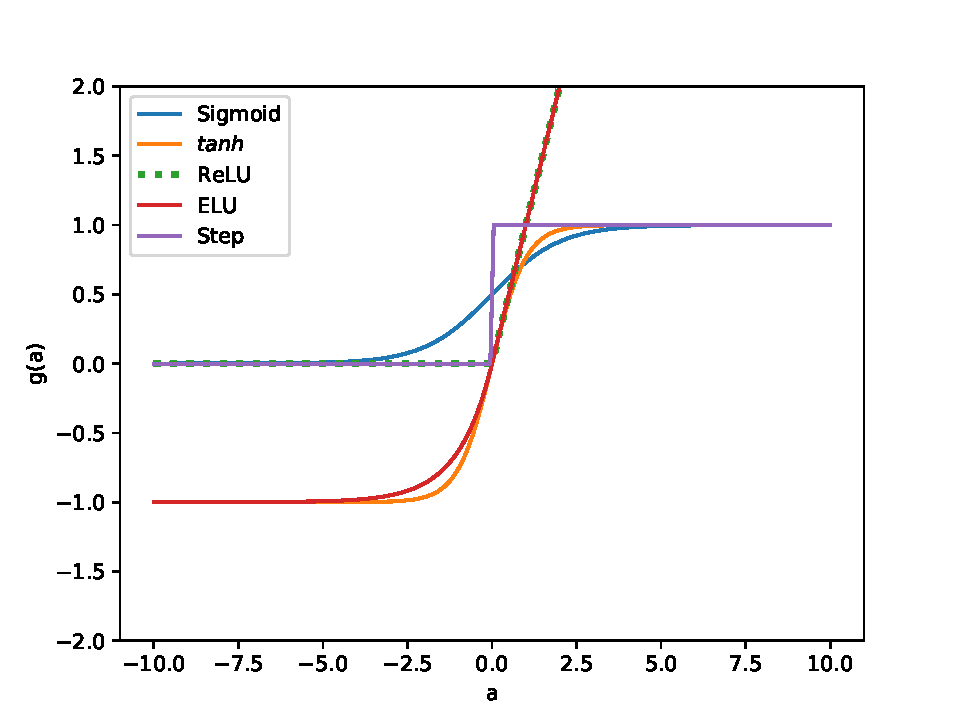
\includegraphics[width=\textwidth,height=\textheight,keepaspectratio]{pics/act_func_fig.pdf}
    \caption{Plot of some of the most used activation functions.}
    \label{fig:act_funcs}
\end{figure}


\section{Backpropagation} \label{sec:backprop}
As mentioned in section \ref{sec:train_val} we seek to find the hypothesis $\hat{h}^*_S$ that minimizes our loss empirical loss. In the case of neural networks (with omitted bias terms) $\hat{h}^*_S$ are the weights used in each neuron as described in section \ref{sec:feedforward_nn}. To obtain these optimal weights we train the neural network by minimizing the gradient of the empirical loss with respect to the weights. To learn these weights we use a minimization algorithm like stochastic gradient descent described in section \ref{sec:sgd}. However the gradient of the loss function is not readily available in neural networks as we have to trace back the information back through the network that produced $\hat{y}$ for which we calculate the loss. The solution is an algorithm proposed by \cite{Rumelhart:1986a} called back-propagation or backprop for short.\\
\\
Back-progatation uses the chain rule of calculus, which states that
\begin{equation*}
    \frac{d \, f\lr{g\lr{x}}}{d \, x} = \frac{d \, f\lr{g\lr{x}}}{d \, g \lr{x}} \frac{d \, g\lr{x}}{d \, x}
\end{equation*}
for a real number $x$ and functions $g$ and $f$. This rule can be generalized to vector 